\documentclass{beamer}
\beamertemplatenavigationsymbolsempty
\usepackage{amsmath, amssymb, hyperref, graphics}
\usepackage{tikz}
\usetikzlibrary{arrows}


\title{Graph Theory Lecture 9}

\begin{document}
\begin{frame}{Today: Shortest and Longest paths}
  But first a basic definition.
  \begin{definition} A \emph{directed graph} is one where each edge has a chosen starting and ending point, usually indicated with arrows.
 \end{definition}
\begin{center}
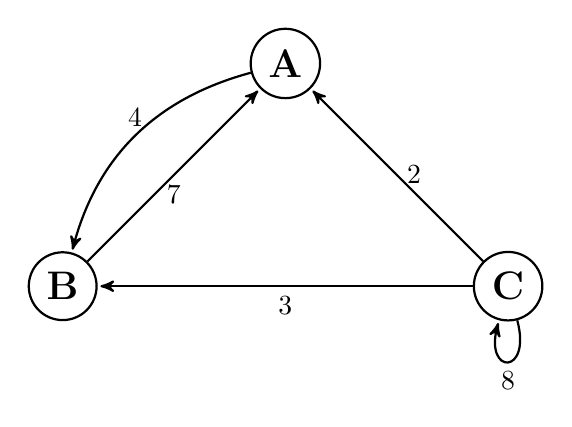
\begin{tikzpicture}[scale=.8,->,>=stealth', shorten >=1pt,auto,node distance=4cm,
                thick,main node/.style={circle,draw,font=\Large\bfseries}]

  \node[main node] (1) {A};
  \node[main node] (2) [below left of=1] {B};
  \node[main node] (3) [below right of=1] {C};

  \path
    (1) edge [bend right] node[above] {4} (2)
    (2) edge node [below]{7} (1)
    (3) edge [loop below] node {8} (3)
        edge node[right] {2} (1)
        edge node[below] {3} (2);      
\end{tikzpicture}
\end{center}


  
  \begin{block}{Walks in directed graphs:}
You can only travel the edge in the direction the arrow shows.
    \end{block}
\end{frame}

\begin{frame}{Dijkstra's algorithm for shortest path}
  \begin{block}{Input:} A weighted (possibly directed) graph $G$ and starting vertex $v\in G$
  \end{block}
  \begin{block}{Output:} For every vertex $w\in G$ a list of all shortest paths from $v$ to $w$
  \end{block}
  
 \begin{block}{Initialize:}
   From starting vertex $v$ list every edge out of $v$ as a poential shortest path to corresponding vertex $w$
   \end{block}
       \begin{block}{Iterate:}
 \begin{itemize}
 \item Choose $w$ with cheapest potential shortest path and make these paths permanent


 \item Update list of potential paths by adding edges out of $w$ to the shortest paths to $w$ and checking if they're cheaper than known paths
   \end{itemize}
 \end{block}
  \end{frame}

\begin{frame}{Example graph from the 2008 Exam}
Find all shortest paths from $S$ to $T$.
\begin{center}
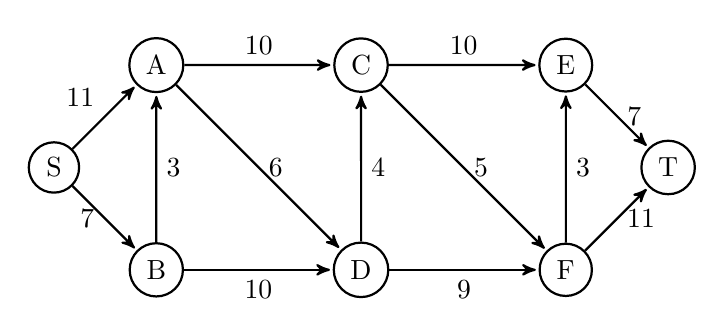
\begin{tikzpicture}[scale=1.3, ->,>=stealth', shorten >=1pt,auto,node distance=4cm,
                thick,main node/.style={circle,draw}]

  \node[main node] (S) at (0,1) {S};
  \node[main node] (A) at (1,2) {A};
  \node[main node] (B) at (1,0) {B};
  \node[main node] (C) at (3,2) {C};
  \node[main node] (D) at (3,0) {D};
  \node[main node] (E) at (5,2) {E};
  \node[main node] (F) at (5,0) {F};
  \node[main node] (T) at (6,1) {T};
  
  \path
    (S) edge node {11} (A)
      edge node[left] {7} (B)
      (B) edge node[below] {10} (D)
      edge node[right] {3} (A)
      (A)       edge node[above] {10} (C)
      edge node[right] {6} (D)
      (C)       edge node[above] {10} (E)
      edge node[right] {5} (F)
      (D)    edge node[right] {4} (C)
      edge node[below] {9} (F)
      (E)      edge node[right] {7} (T)
      (F)      edge node[right] {11} (T)
            edge node[right] {3} (E);
\end{tikzpicture}
\end{center}

\begin{block}{Add on:}
\begin{itemize}
\item  Which edges if made a little longer would make the distance from $S$ to $T$ longer?
\item  Which edges if made a little shorter would make the distance from $S$ to $T$ shorter?
\end{itemize}
\end{block}

  \end{frame}


\begin{frame}{The main idea of why Dijkstra's works:}


Suppose we're at the step were Dijkstra's decides the cheapest path to $w$. 
\begin{block}{Then:}
A cheaper path to $w$ would have to go through a vertex $u$ we haven't found the cheapest path to yet.
  \end{block}

  \begin{block}{But!}
Even \emph{getting} to $u$ costs more than our cheapest path to $w$.
    \end{block}

  \begin{block}{An observation:}
Dijkstra's algorithm depends on the edge weights being non-negative!
  \end{block}
  
  \end{frame}

\begin{frame}{Culture: performance of Dijkstra's algorithm}
  \begin{block}{In a limited sense, Dijkstra's algorithm is optimal:}
If \emph{all we know} is that we have a weighted graph, then you can't do better than Dijkstra's algorithm.
    \end{block}
  \begin{block}{In practise, often not very good:}
 When finding path from Sheffield to Edinburgh, Dijkstra's algorithm explores every street in London.
  \end{block}
  \begin{block}{Real world maps have extra information:}
    It's easy to calculate the distance between two points as the crow flies, and we know the driving distance has to be at least that large.  
\end{block}  
  \begin{block}{The A* algorithm avoids searching London:}
    Supposes we have an easy to calculate ``heuristic distance'' $h(v,w)$, that is a lower bound for the actual distance $d(v,w)$. 
    \end{block}
\end{frame}


\begin{frame}{Finding the longest path}
  \begin{block}{Scheduling a large problem with many parts}
For example, building a house.
    \begin{itemize}
    \item Some can be done at same time: (finishing interior rooms)
    \item Some need to be done in order: (foundation before walls)
    \item How early could whole project be finished?
    \end{itemize}
  \end{block}
  \begin{block}{Solution: longest path}
    \begin{itemize}
    \item  Encode tasks as edges in directed weighted graph        
    \item Edge $e$ follows edge $f$ if task $f$ requires task $e$ 
    \item Length of longest path is the shortest time to complete project 
    \end{itemize}
\end{block}
Building the directed graph from a list of tasks and dependencies can require a few tricks and won't be tested.

\end{frame}

\begin{frame}{Longest path might not exist:}

  \begin{block}{A necessary assumption:}
    If the graph has a directed cycle, we could get an infinitely long path by repeating graph over and over again.  
  \end{block}

  \begin{definition}A directed graph $G$ is \emph{acyclic} if it has no directed cycles.
  \end{definition}

  \begin{block}{Graphs in scheduling applications are acyclic:}
 Otherwise we'd have a cycle of tasks that all depend on each other and we could never start the project!  
\end{block}

  \begin{block}{Ordering vertices / ``topological sort''}
    If $G$ is acyclic it's easy to order the vertices of $G$ so that if there's an edge from $v$ to $w$, then $w$ comes after $v$.
\end{block}
\end{frame}

\begin{frame}{The longest path algorithm:}
\begin{block}{Initializing:}
  \begin{itemize}
    \item Topologically sort the vertices of $G$ 
    \item List every edge of starting vertex as potential longest path
  \end{itemize}
\end{block}

\begin{block}{Iterate:}
  \begin{itemize}
  \item Make the potential longest path to the first vertex $w$  on the list permament
  \item Update the list of potential longest paths adding edges out of $w$ to longest paths to $w$ and seeing if they create new longest paths
  \end{itemize}
  \end{block}
  
  

  
  \end{frame}


\begin{frame}{Example graph from the 2008 Exam}
Find all longest paths from $S$ to $T$.
\begin{center}
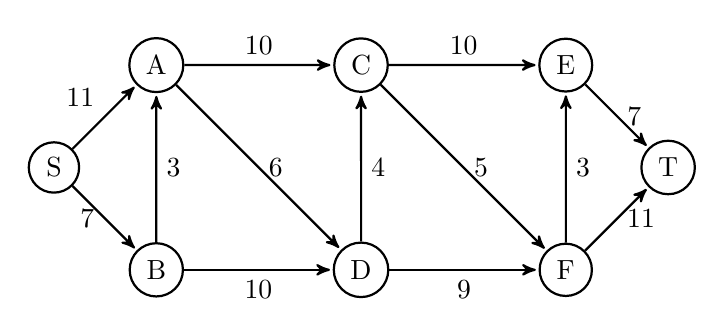
\begin{tikzpicture}[scale=1.3, ->,>=stealth', shorten >=1pt,auto,node distance=4cm,
                thick,main node/.style={circle,draw}]

  \node[main node] (S) at (0,1) {S};
  \node[main node] (A) at (1,2) {A};
  \node[main node] (B) at (1,0) {B};
  \node[main node] (C) at (3,2) {C};
  \node[main node] (D) at (3,0) {D};
  \node[main node] (E) at (5,2) {E};
  \node[main node] (F) at (5,0) {F};
  \node[main node] (T) at (6,1) {T};
  
  \path
    (S) edge node {11} (A)
      edge node[left] {7} (B)
      (B) edge node[below] {10} (D)
      edge node[right] {3} (A)
      (A)       edge node[above] {10} (C)
      edge node[right] {6} (D)
      (C)       edge node[above] {10} (E)
      edge node[right] {5} (F)
      (D)    edge node[right] {4} (C)
      edge node[below] {9} (F)
      (E)      edge node[right] {7} (T)
      (F)      edge node[right] {11} (T)
            edge node[right] {3} (E);
\end{tikzpicture}
\end{center}

\begin{block}{Add on:}
\begin{itemize}
\item  Which edges if made a little longer would make the longest path from $S$ to $T$ longer?
\item  Which edges if made a little shorter would make the longest path from $S$ to $T$ shorter?
\end{itemize}
\end{block}

  \end{frame}
  


\end{document}
